\documentclass[12pt,a4paper]{article}

\usepackage[in, plain]{fullpage}
\usepackage{array}
\usepackage{../../../moncours2}


%\usepackage{pas-cours}
%%-------------------------------------------------------------------------------
%          -Packages nécessaires pour écrire en Français et en UTF8-
%-------------------------------------------------------------------------------
\usepackage[utf8]{inputenc}
\usepackage[frenchb]{babel}
\usepackage[T1]{fontenc}
\usepackage{lmodern}
\usepackage{textcomp}



%-------------------------------------------------------------------------------

%-------------------------------------------------------------------------------
%                          -Outils de mise en forme-
%-------------------------------------------------------------------------------
\usepackage{hyperref}
\hypersetup{pdfstartview=XYZ}
%\usepackage{enumerate}
\usepackage{graphicx}
\usepackage{multicol}
\usepackage{tabularx}
\usepackage{multirow}


\usepackage{anysize} %%pour pouvoir mettre les marges qu'on veut
%\marginsize{2.5cm}{2.5cm}{2.5cm}{2.5cm}

\usepackage{indentfirst} %%pour que les premier paragraphes soient aussi indentés
\usepackage{verbatim}
\usepackage{enumitem}
\usepackage[usenames,dvipsnames,svgnames,table]{xcolor}

\usepackage{variations}

%-------------------------------------------------------------------------------


%-------------------------------------------------------------------------------
%                  -Nécessaires pour écrire des mathématiques-
%-------------------------------------------------------------------------------
\usepackage{amsfonts}
\usepackage{amssymb}
\usepackage{amsmath}
\usepackage{amsthm}
\usepackage{tikz}
\usepackage{xlop}
%-------------------------------------------------------------------------------



%-------------------------------------------------------------------------------


%-------------------------------------------------------------------------------
%                    - Mise en forme avancée
%-------------------------------------------------------------------------------

\usepackage{ifthen}
\usepackage{ifmtarg}


\newcommand{\ifTrue}[2]{\ifthenelse{\equal{#1}{true}}{#2}{$\qquad \qquad$}}

%-------------------------------------------------------------------------------

%-------------------------------------------------------------------------------
%                     -Mise en forme d'exercices-
%-------------------------------------------------------------------------------
%\newtheoremstyle{exostyle}
%{\topsep}% espace avant
%{\topsep}% espace apres
%{}% Police utilisee par le style de thm
%{}% Indentation (vide = aucune, \parindent = indentation paragraphe)
%{\bfseries}% Police du titre de thm
%{.}% Signe de ponctuation apres le titre du thm
%{ }% Espace apres le titre du thm (\newline = linebreak)
%{\thmname{#1}\thmnumber{ #2}\thmnote{. \normalfont{\textit{#3}}}}% composants du titre du thm : \thmname = nom du thm, \thmnumber = numéro du thm, \thmnote = sous-titre du thm

%\theoremstyle{exostyle}
%\newtheorem{exercice}{Exercice}
%
%\newenvironment{questions}{
%\begin{enumerate}[\hspace{12pt}\bfseries\itshape a.]}{\end{enumerate}
%} %mettre un 1 à la place du a si on veut des numéros au lieu de lettres pour les questions 
%-------------------------------------------------------------------------------

%-------------------------------------------------------------------------------
%                    - Mise en forme de tableaux -
%-------------------------------------------------------------------------------

\renewcommand{\arraystretch}{1.7}

\setlength{\tabcolsep}{1.2cm}

%-------------------------------------------------------------------------------



%-------------------------------------------------------------------------------
%                    - Racourcis d'écriture -
%-------------------------------------------------------------------------------

% Angles orientés (couples de vecteurs)
\newcommand{\aopp}[2]{(\vec{#1}, \vec{#2})} %Les deuc vecteurs sont positifs
\newcommand{\aopn}[2]{(\vec{#1}, -\vec{#2})} %Le second vecteur est négatif
\newcommand{\aonp}[2]{(-\vec{#1}, \vec{#2})} %Le premier vecteur est négatif
\newcommand{\aonn}[2]{(-\vec{#1}, -\vec{#2})} %Les deux vecteurs sont négatifs

%Ensembles mathématiques
\newcommand{\naturels}{\mathbb{N}} %Nombres naturels
\newcommand{\relatifs}{\mathbb{Z}} %Nombres relatifs
\newcommand{\rationnels}{\mathbb{Q}} %Nombres rationnels
\newcommand{\reels}{\mathbb{R}} %Nombres réels
\newcommand{\complexes}{\mathbb{C}} %Nombres complexes


%Intégration des parenthèses aux cosinus
\newcommand{\cosP}[1]{\cos\left(#1\right)}
\newcommand{\sinP}[1]{\sin\left(#1\right)}


%Probas stats
\newcommand{\stat}{statistique}
\newcommand{\stats}{statistiques}
%-------------------------------------------------------------------------------

%-------------------------------------------------------------------------------
%                    - Mise en page -
%-------------------------------------------------------------------------------

\newcommand{\twoCol}[1]{\begin{multicols}{2}#1\end{multicols}}


\setenumerate[1]{font=\bfseries,label=\textit{\alph*})}
\setenumerate[2]{font=\bfseries,label=\arabic*)}


%-------------------------------------------------------------------------------
%                    - Elements cours -
%-------------------------------------------------------------------------------





%\makeatletter
%\renewcommand*{\@seccntformat}[1]{\csname the#1\endcsname\hspace{0.1cm}}
%\makeatother

%\toggletrue{eleve}
%\toggletrue{dys}

\date{}
\title{\textcircled{{\normalsize{3}}}Addition, soustraction et multiplication }

\renewcommand{\labelitemi}{∙}
%
%\rfoot{Page \thepage}
\begin{document}
%
%\dominitoc
%
%\tableofcontents

\maketitle

%\chapter{Droites, segments et codage}

%
\begin{myobj}
	\begin{itemize}
		
		\item Construire le symétrique d’un point ou d'une figure par rapport à une droite à la main où à l’aide d’un logiciel;
		\item Construire le symétrique d’un point ou d'une figure par rapport à un point, à la main où à l’aide d’un logiciel;
		\item Utiliser les propriétés de la symétrie axiale ou centrale;
		\item Identifier des symétries dans des figures.		
	\end{itemize}
\end{myobj}

\begin{mycomp}
	\begin{itemize}
		\item \kw{Chercher (Ch2)} :  s’engager    dans    une    démarche    scientifique, observer, questionner, manipuler, expérimenter (sur une feuille de papier, avec des objets, à l’aide de logiciels), émettre des hypothèses, chercher des exemples ou des contre-exemples, simplifier ou particulariser une situation, émettre une conjecture ;
		\item \kw{Raisonner (Ra3)} :  démontrer : utiliser un raisonnement logique et des règles établies (propriétés, théorèmes, formules) pour parvenir à une conclusion ;
		\item \kw{Communiquer (Co2)} :  expliquer à l’oral ou à l’écrit (sa démarche, son raisonnement, un calcul, un protocole   de   construction   géométrique, un algorithme), comprendre les explications d’un autre et argumenter dans l’échange ; 
		
	\end{itemize}
\end{mycomp}



%
\section{Additionner et soustraire}
%
\begin{mymeth}
	Pour additionner ou soustraire deux fractions :
	
	\begin{enumerate}
		\item Je les écrit avec le \kw{même dénominateur};
		\item Je fais la \kw{somme des numérateurs};
		\item Je ne modifie pas le dénominateur;
	\end{enumerate}
\end{mymeth}

\begin{myexs}
	\begin{multicols}{3}
	
	
				\begin{eqnarray*}
					A &=& \frac{3}{5} + \frac{1}{5} \\
					A &=& \frac{3 + 1}{5}\\
					A &=& \frac{4}{5}\\
				\end{eqnarray*}
			
	
			\begin{eqnarray*}
				B &=& \frac{14}{3} - 2 \\
				B &=& \frac{14}{3} - \frac{2 \times 3}{3}\\
				B &=& \frac{14}{3} - \frac{6}{3}\\
				B &=& \frac{14 - 6}{3}\\				
				B &=& \frac{8}{3}\\
			\end{eqnarray*}
	
			\begin{eqnarray*}
				C &=& \frac{2}{3} + \frac{4}{9} \\
				C &=& \frac{2 \times 3}{3 \times 3} + \frac{4}{9}\\
				C &=& \frac{6}{9} + \frac{4}{9}\\
				C &=& \frac{6 + 4}{9}\\
				C &=& \frac{10}{9}\\
			\end{eqnarray*}
	
	\end{multicols}
\end{myexs}

\newpage

\section{Multiplier}

\begin{mydef}
			Un \kw{produit} est le résultat de la \kw{multiplication} de deux \kw{facteurs}.
		
\end{mydef}
	
\begin{myex}
	\begin{center}
		\includegraphics*[scale=0.7]{img/produit}
	\end{center}
\end{myex}

\begin{myprop}
	Dans une multiplication, \kw{l'ordre des facteurs n'a pas d'importance}.
\end{myprop}

\begin{myex}
	\begin{itemize}
		\item $4 \times 2 \times 5 = 2 \times 5 \times 4 = 10 \times 4 = 40$
		\item $\num{3.5} \times \num{2.5} \times 4 \times \num{2} = \num{3.5} \times \num{2} \times 4 \times \num{2.5} = 7 \times 10 = 70$
	\end{itemize}
\end{myex}

\section{Priorité des opérations}

\section{Calcul d'expressions}

\begin{questions}
	\question Calculer les expressions suivantes en détaillant toutes les étapes du calcul.
	\begin{multicols}{2}
		\begin{parts}
			\part $A = \num{7.25} + \num{6.1} + \num{5.75} + \num{3.9}$
			\begin{solution}
				\begin{eqnarray*}
					A &=& \num{7.25} + \num{6.1} + \num{5.75} + \num{3.9} \\
					A &=& \num{7.25} + \num{5.75} + \num{6.1} + \num{3.9} \\
					A &=& 13 + 10 \\
					A &=& 23 
				\end{eqnarray*}
			\end{solution}
			
			\part $B = 25 + 5 \times 8$
			\begin{solution}
				\begin{eqnarray*}
					B &=& 25 + 5 \times 8 \\
					B &=& 25 + 40 \\
					B &=& 65 \\
				\end{eqnarray*}
			
				\vspace*{0.5cm}
			\end{solution}
		
			\part $C = 4 + 6 \times 3 + \num{6.25} \times 4$
			\begin{solution}
				\begin{eqnarray*}
					C &=& 4 + 6 \times 3 + \num{6.25} \times 4 \\
					C &=& 4 + 18 + 25 \\
					C &=& 22 + 25 \\
					C &=& 47 
				\end{eqnarray*}
			\end{solution}
		
			\part $D = \num{3.5} \times (9 + \num{4.5} + \num{2.3}$
			\begin{solution}
				\begin{eqnarray*}
					D &=& \num{3.5} \times (9 + \num{4.5} + \num{2.3}) \\
					D &=& \num{3.5} \times (9 + \num{6.8}) \\
					D &=& \num{3.5} \times  \num{15.8} \\
					D &=& \num{55.3} 
				\end{eqnarray*}
			\end{solution}
		\end{parts}
	\end{multicols}	
	

	\question Rajouter des parenthèse (uniquement celles qui sont indispensables) pour que les égalités soient correctes. Vérifier en détaillant le calcul.
	
	\begin{parts}
		\begin{multicols}{2}
			\part $1 + 4 \times 6 = 30$
			\begin{solution}
				\begin{eqnarray*}
					(1 + 4) \times 6 &=& 5 \times 6 \\
					(1 + 4) \times 6 &=& 30 
				\end{eqnarray*}
			\end{solution}
			
			\part $34 - 12 + 22 = 0$
			\begin{solution}
				\begin{eqnarray*}
					34 - (12 + 22) &=& 34 - 34 \\
					34 - (12 + 22) &=& 0 
				\end{eqnarray*}
			\end{solution}
		
			\part $17 - 4 \times 4 = 2 \times 17 + 9$
			\begin{solution}
				\begin{eqnarray*}
					(17 - 4) \times 4 &=& 13 \times 4 \\
					(17 - 4) \times 4  &=& 52 
				\end{eqnarray*}
			
				\begin{eqnarray*}
					2 \times (17 + 9) &=& 2 \times 26 \\
					2 \times (17 + 9)  &=& 53 
				\end{eqnarray*}
			\end{solution}
		
			\part $4 + 5 \times 6 + 3 = 81$
			\begin{solution}
				\begin{eqnarray*}
					(4 + 5) \times (6 + 3) &=& 9 \times 9 \\
					(4 + 5) \times (6 + 3) &=& 81 
				\end{eqnarray*}
			\end{solution}	
		\end{multicols}
		
	\end{parts}
\end{questions}




%
%\newpage
%
%\section{Longueurs et codages}
%
%\begin{mydefs}
	\iftoggle{eleve}{%
		La mesure \hrulefill
		
		\vspace*{0.2cm}
		\hrulefill 
		
		La longueur \hrulefill
		
	}{%
	La mesure d'un segment (distance entre ses deux extrémités) est sa \kw{longueur}.
	
	La longueur d'un segment $[AB]$, se note $AB$ ou $BA$. 
}
\end{mydefs}


\begin{myex}
	\vspace*{-0.5cm}
	\begin{center}
		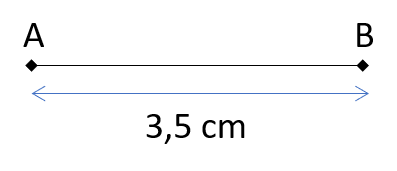
\includegraphics[scale=0.8]{img/lgr}
	\end{center}
	\vspace*{-0.5cm}
	
	\iftoggle{eleve}{%
		La longueur \hrulefill
		\vspace*{0.2cm}
		\hrulefill 
}{%
	La longueur du segment $[AB]$ est de \num{3.5} cm, on note $AB=\num{3.5}$ cm.
}	
	
\end{myex}

\begin{mydef}
	\iftoggle{eleve}{%
		Le \kw{milieu} d'un segment \hrulefill \\
		\vspace*{0.2cm}
		\hrulefill 
	}{%
		Le \kw{milieu} d'un segment est le point qui appartient au segment \kw{et} qui est à égale distance de ses extrémités.
	}
	
\end{mydef}

\begin{myrem}
	\iftoggle{eleve}{%
		Des segments de \hrulefill 
		
		\vspace*{0.2cm}
		\hrulefill 
	}{%
		Des segments de même longueur sont codés de façon identique.
	}
	
\end{myrem}

\begin{myex}
	
	\begin{center}
		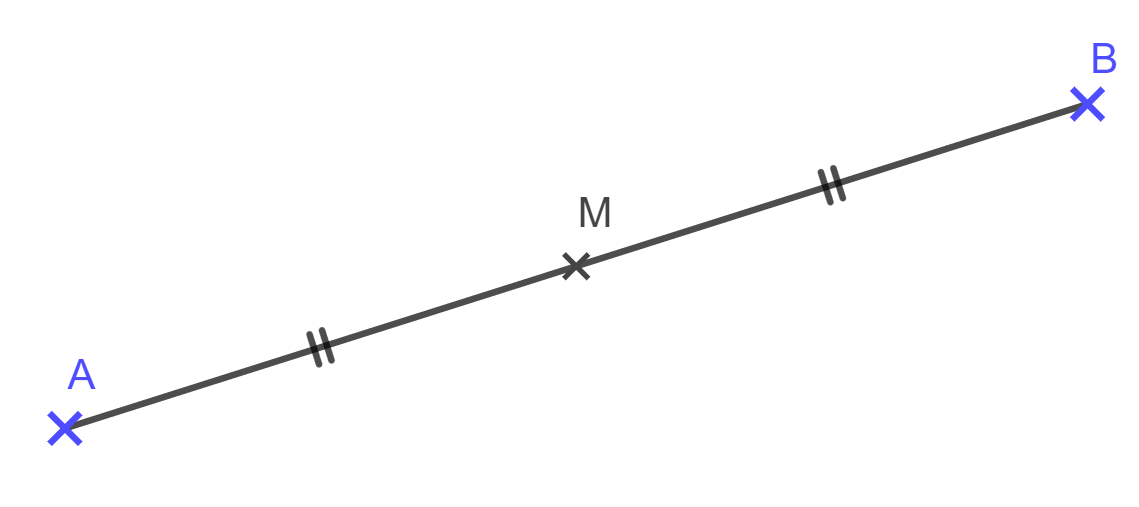
\includegraphics[scale=0.35]{img/milieu}
	\end{center}
	\iftoggle{eleve}{%
		On a : $M \in [AB]$ \hrulefill 
		
		\vspace*{0.2cm}
		\hrulefill 
	}{%
		On a : $M \in [AB]$ et $AM = MB$, donc le point $M$ est le milieu du segment $[AB]$. On a ainsi $AM = AB \div 2$. 
	}

\end{myex}
%
%\section{Sécantes, perpendiculaires et parallèles}


\end{document}